In this question, we will guide you through how to apply nodes and resistance equivalence to solve a complex resistor network (like the cubic one above, assuming all resistors are identical with a resistance of $R$) and find the equivalent resistance between the top back left node and the bottom front right node. \\
\note{For this question, encourage the students to follow through the questions and apply nodal analysis and equivalent resistance along the way. Assure them that with the symmetrical nature of this cubic network, the result will appear less complicated than they expect.}

\begin{figure}[H]
    \centering
    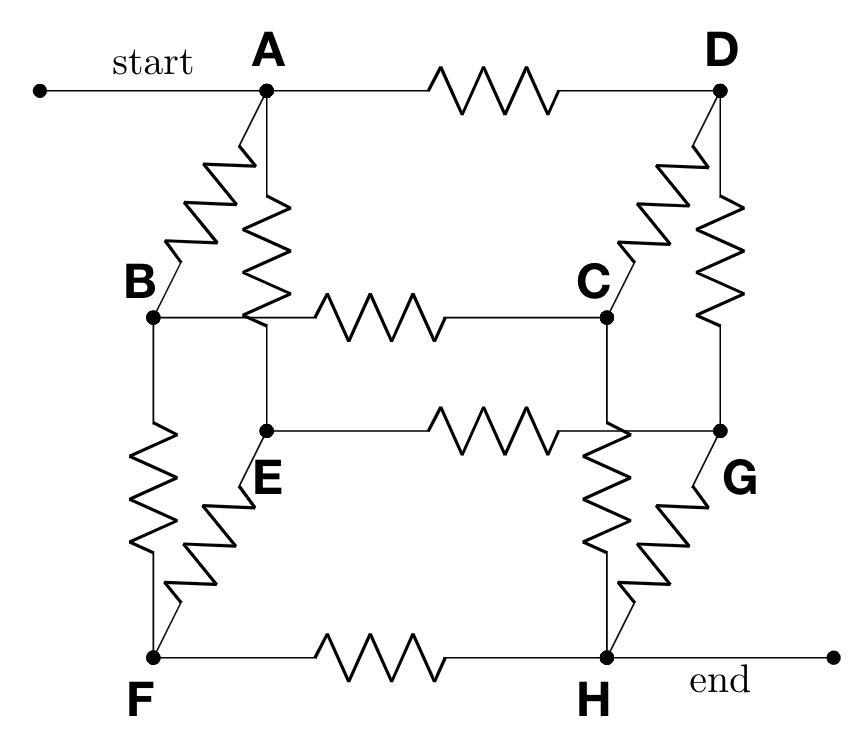
\includegraphics[scale=0.45]{../labeled.png}
    \caption{3D View of the Resistor Network}
\end{figure}

\begin{figure}[H]
    \centering
    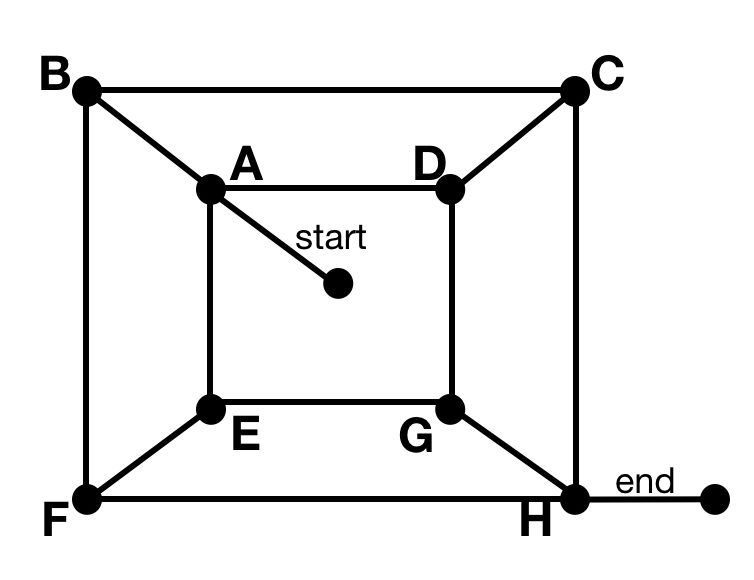
\includegraphics[scale=0.45]{../flattened.png}
    \caption{Flattened View of the Resistor Network, \\ where each segment between 2 nodes has a resistance of $R$}
\end{figure}

\begin{enumerate}
    \item As daunting as this question looks, fortunately we have the power of nodal analysis on our side! To get started, group the vertices from $B$ through $H$ based on the \textbf{distances of the shortest paths} along the edges of the cube starting from $A$. For example, the distance of the shortest path from $A$ to the bottom front left vertex will be 2 (assuming each edge of the cube is 1 unit long). \\
    \note{Make sure to clarify to the students that shortest path always starts from $A$ (as our point of departure) and must go along the edges of the cube.} \\
    \sol{
        Starting from the vertex $A$, we can see that:
        $B$, $D$, and $E$ are all 1 unit away from $A$, while $F$, $G$, abd $C$ are 2 units away from $A$, and $H$ (the endpoint) is 3 units away from $A$.
    }
    \item Now, consider the group of all the vertices $v_i$ that are 1 unit away from $A$ (the starting node in the top back left) and the resistors in and between these pairs of nodes ($v_i$, $A$). How are they related to each other (Hint: think in terms of equivalent resistance)? \\
    \note{For this part, encourage the students to think in terms of potential differences. Use the following scenario as an example to provide them with some helpful hints: \\
    Suppose I have 2 pairs of nodes $(A, B)$ and $(C, D)$, both pairs have the same resistances between them $R_{A-B} = R_{C-D}$. What can we conclude about the potential differences ($V_{A-B}, V_{C-D}$) of both pairs?
    } \\
    \sol{Based on our labeling convention in the previous part, the nodes that are 1 unit away from $A$ are $B$, $D$, and $E$. Since all these nodes are of the same distance away from the starting node $A$, and the resistance between these nodes and $A$ is the same ($R$), the potential differences between $A$ and these nodes are \textbf{all the same}! This means that the 3 resistors between $A$ and the nodes that are 1 unit away from it are in parallel.}
    \item Now, consider the group of all the vertices $v_j$ that are 2 units away from $A$. Call it Group II. Let the group in the previous part be Group I. How many edges lead from a vertex in Group I to a vertex in Group II (how many resistors are involved in this case)? \\
    \sol{To count how many edges lead from a vertex in Group I to a vertex in Group II, we can begin with any vertex from the set $\{B, D, E \}$ and count the number of distinct edges that lead from it 1 unit farther away from $A$. As we can see in the cube above, for each vertex $v_i$ in Group I, there are exactly 2 distinct edges that lead to a vertex 1 unit farther away from $A$. So, there are $3 \times 2 = 6$ such edges in total. Since each edge contains a resistor, there are 6 resistors involved in total.}
    \item How are Group I and Group II related with each other? Is there anything we can do to simplify the resistor network so far? \\

    \note{When teaching, encourage the students to think about the following questions before working on this part:

    \begin{itemize}
        \item What happens if you merge the vertices(nodes) with the same potentials into one?
        \item How can we apply this to Group I, Group II and the resistors involved in both groups?
    \end{itemize}
    }

    \sol{
        When we have nodes with the same potential, if we merge them into one, the overall potential difference between the merged endpoint and $A$ still remains the same. This implies that merging all nodes with the same potential into one junction won't affect the overall structure or resistance of this resistor network!
        
        Since nodes in Group II are 1 unit away from the nodes in Group I, and similarly, all resistors in and between are in parallel as well, we can merge their start nodes and end nodes into a single junction as well! Therefore, the overall resistors between the vertices in Group I and $A$ are in series with those between the vertices in Group I and the vertices in Group II. So essentially, we have 3 resistors (from Group I) in parallel, and overall in series with 6 resistors (between Group I and Group II) in parallel.
    }
    \item Finally, How far away is $H$ (the ending node) from $A$ (the starting node)? How many edges are there that lead from the nodes in Group II to $H$? Using equivalent resistance, is there anyway we can simplify all the circuits along the edges from the nodes in Group II to $H$? (Hint: think in terms of symmetry and what you've found in part (b)) \\
    \sol{Here comes the symmetrical beauty that underlines this cubic network! If we rotate the entire cubic resistor network by 180 degrees about the space diagonal from $A$ and $H$, we will exactly end up with $A$ swapped with $H$. What this really means is that all the edges that lead from the vertices in Group II to $H$ are equivalent to the edges that first extend 1 unit away from $A$ in part (b)! This further implies that the 3 resistors along these edges are in parallel again (as we converge back onto one end node)!}
    \item Combining all your findings together, what is the overall resistance between the starting node on the top back left and the ending node on the bottom front right in this cubic resistor network? \\
    \note{For the final part, encourage the students to try "flattening" the 3D resistor network onto a plane. Make sure to bring up how they can apply all the resistance equivalence they've discovered over the previous parts to map out all the resistors based on the nodes and their shortest distances from $A$.} \\
    \sol{
    Let's recap what we've known so far, go through the groups of nodes and the resulting junctions that we merged from the previous parts.
    \begin{enumerate}
        \item Starting from $A$, we have 3 resistors in parallel. Over a distance of 1 unit, we reach the nodes $B, D, E$ in Group I. By the equivalent resistance in a parallel circuit, the overall resistance of these 3 resistors is $\frac{R}{3}$.
        \item Between Group I and Group II, since the distance in and between the vertices from the 2 groups is the same (= 1 unit), and each edge carries the same resistor, this means all edges share the same potentials, therefore, we can merge all the start nodes into one junction $T_0$, and all the end nodes into another junction $T_1$. $T_0$ will contain the vertices $B, D, E$, and $T_1$ will contain the vertices $C, F, G$. Overall between the merged junctions, we have 6 edges (or resistors) in parallel with each other. Therefore, the overall resistance of this part will be $\frac{R}{6}$
        \item Between Group II and the end node $H$, by symmetry from part(e), we can apply what we've done exactly for Group I and $A$. Hence, the overall resistance of this part will be again $\frac{R}{3}$.
        \item All these 3 parts are in series with each other (from $A$ to $H$), hence, by the equivalent resistance of a series circuit, the total resistance between $A$ and $H$ is equal to 
        $$ \frac{R}{3} + \frac{R}{6} + \frac{R}{3} = \frac{5}{6}R$$
        Again, with the power of nodal analysis and equivalent resistance, anything is possible! $\square$
    \end{enumerate}
    }
\end{enumerate}